\documentclass[11pt,a4paper]{article}
\usepackage[utf8]{inputenc}
\usepackage[english]{babel}
\usepackage{amsmath}
\usepackage{amsfonts}
\usepackage{amssymb}
\usepackage{graphicx, wrapfig}
\usepackage[left=2cm,right=2cm,top=2cm,bottom=2cm]{geometry}
\usepackage[hidelinks]{hyperref}
\usepackage{url}
\usepackage{listings}
\usepackage{color}
\usepackage{enumitem}
\usepackage{courier}
\usepackage[bottom]{footmisc}
\usepackage{caption}
\captionsetup{font={small,sf}} % For caption fonts
\captionsetup[sub]{font={small,sf}} % For caption fonts
\usepackage{textcomp}
\usepackage{titling}
\usepackage{tcolorbox}

\setlength{\droptitle}{-2cm}   

\title{\textbf{Assignment 6: Final Programming Project} \\ \Large Advanced Machine Learning Proseminar, Winter Semester 2019-20}
\date{}

\begin{document}
\maketitle

\vspace{-1cm}

\noindent
% Put name and c-number of first member
\textbf{Name/C-number:Raoul Schikora/csav8467}  \\
\textbf{Name/C-number:Oliver Roß/csaq8749}  \\

\section{Answers}

\begin{enumerate}
\item Answer to question 1
	
We used a polynomial degree of 3. The higher the degree the more complex features can be learned. Choosing a very low $n$ would ignore complex interactions. $n>3$ turned out to be not feasible on our laptops or Google Colab in a reasonable amount of time, since it is exponential in $n$.

\item Answer to question 2 (include 3 figures)

We trained our LFA Policy Agent with a discount factor $\gamma = 0.9$, a step size $\alpha = 0.02$ and $n = 3$ for 1000 episodes.
	Figures \ref{fig:1} through \ref{fig:3} show the reward per episode during training.
	\begin{figure}
	\begin{center}
		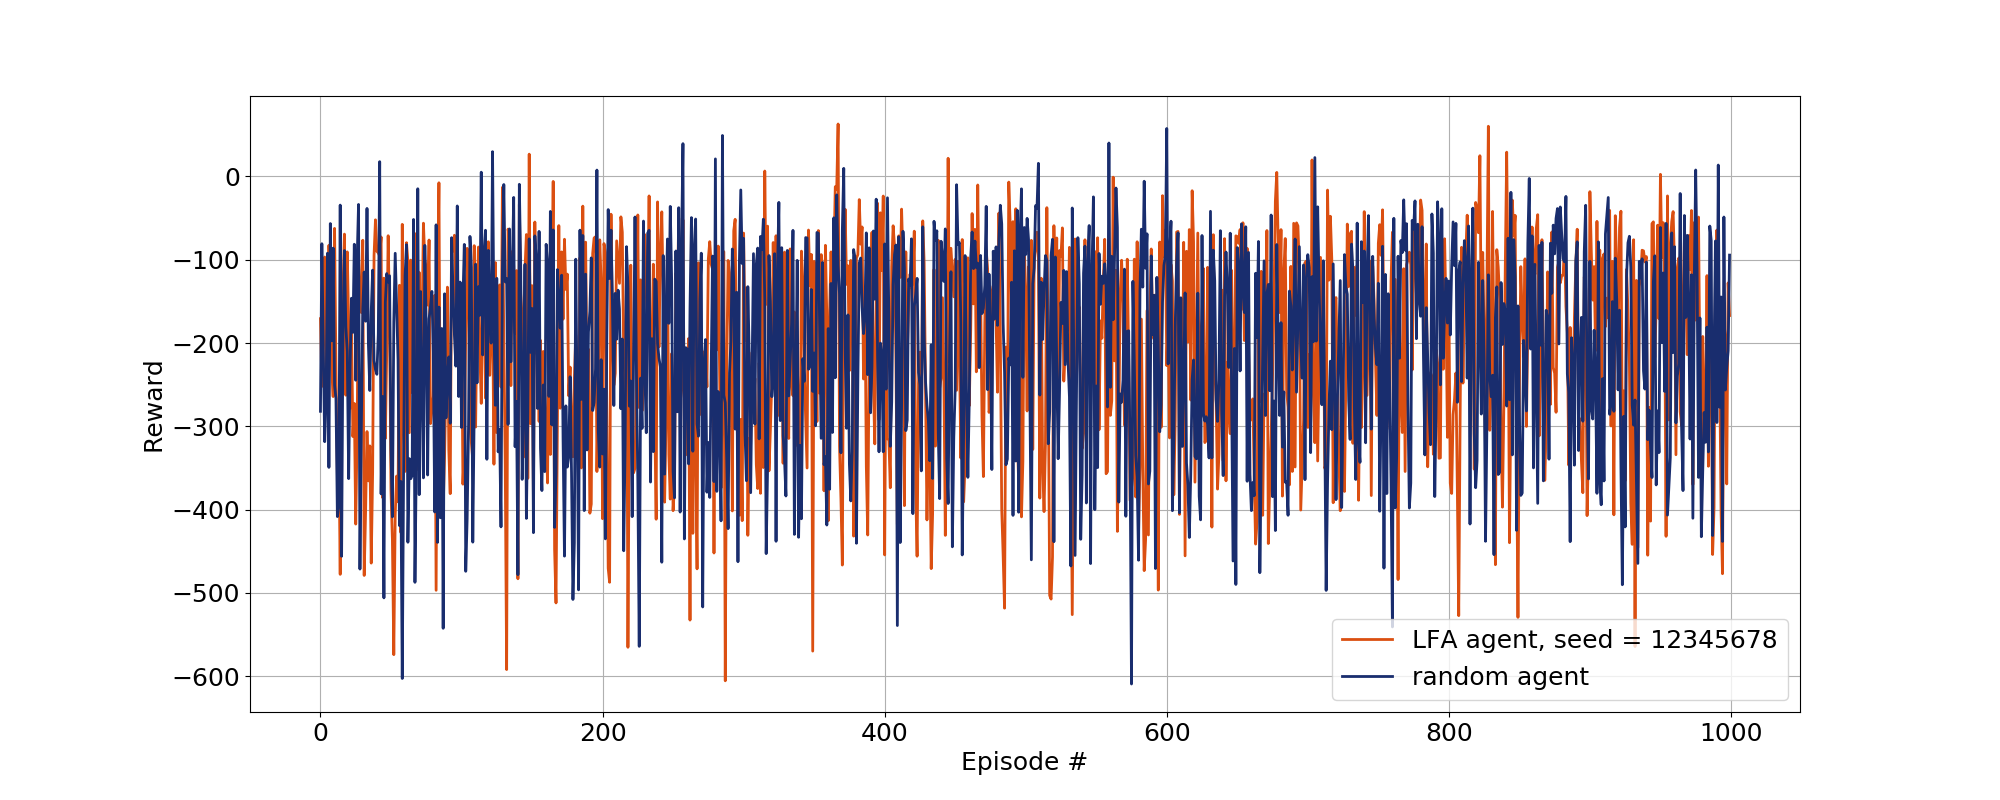
\includegraphics[width = 20cm]{12345678.png}
		\caption{LFA Policy Agent, trained with random seed 12345678. Episode rewards during training.}
		\label{fig:1}
	\end{center}
	\end{figure}

	\begin{figure}
	\begin{center}
		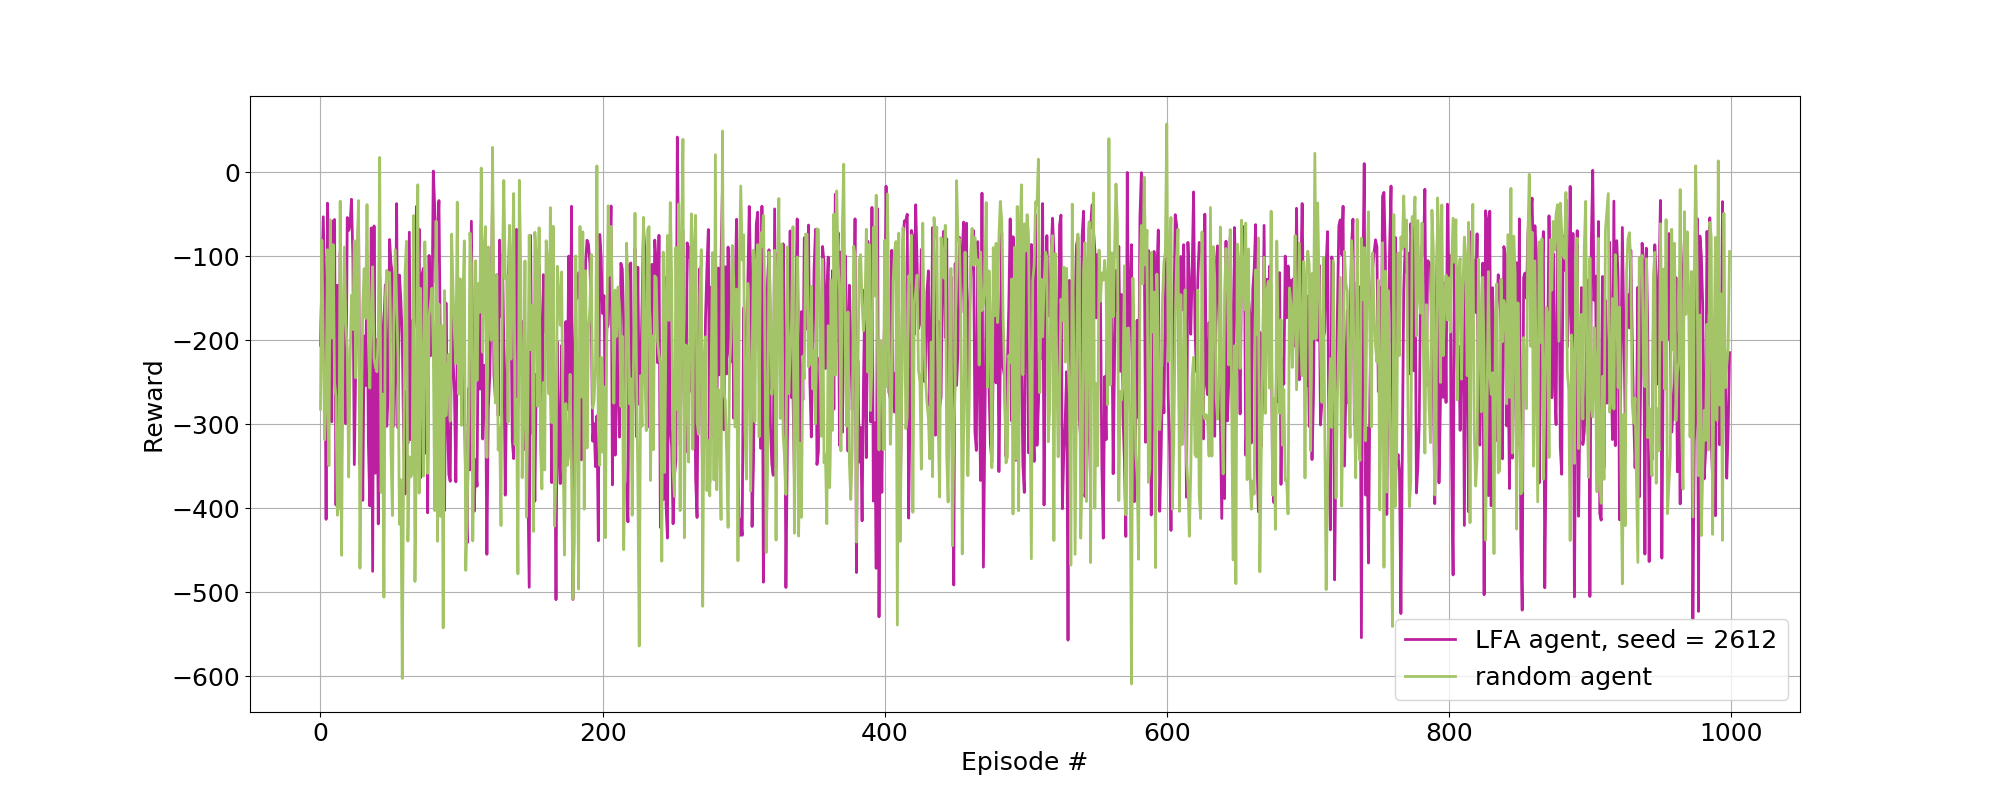
\includegraphics[width = 20cm]{2612.png}
		\
		\caption{LFA Policy Agent, trained with random seed 2612. Episode rewards during training.}
		\label{fig:2}
	\end{center}
	\end{figure}
	\begin{figure}
	\begin{center}
		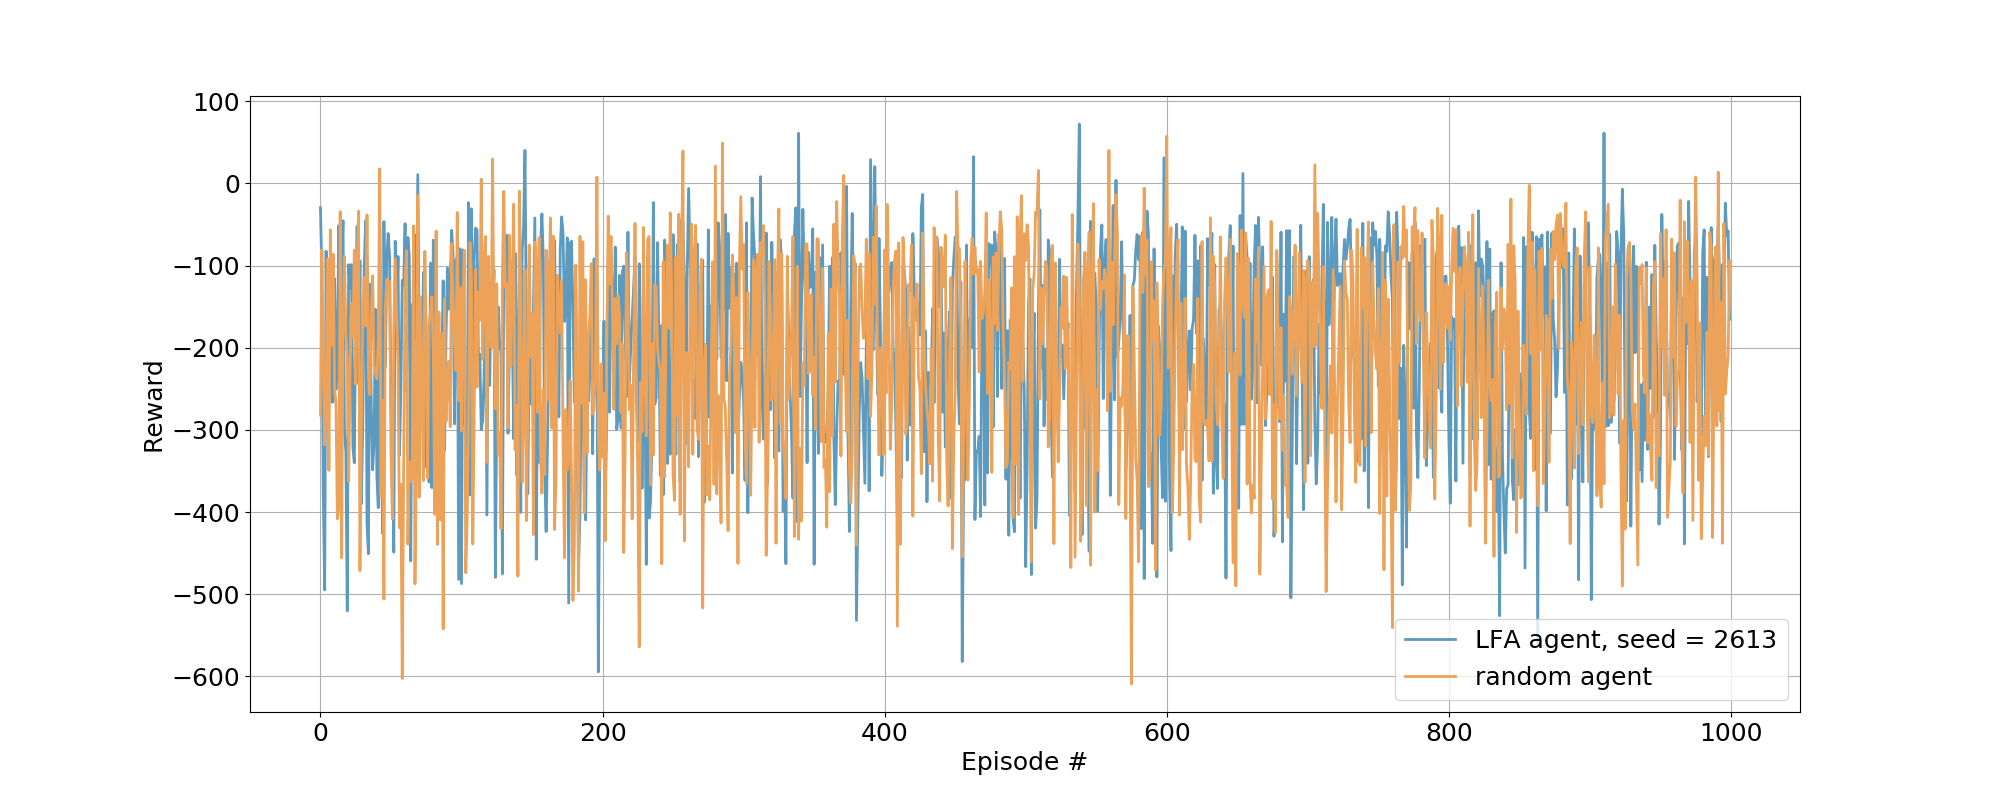
\includegraphics[width = 20cm]{2613.png}
		\caption{LFA Policy Agent, trained with random seed 2613. Episode rewards during training.}
		\label{fig:3}
	\end{center}
	\end{figure}
\item Answer to question 3 
	
Our agent didn't perform significantly better than the random agent. When evaluating the policy after it was learned, with deterministically chosen actions (instead of sampled from a gaussian), we observed slightly better performance and less variance compared to the random agent(see figure \ref{fig:4}). Varying the learning rate from $10^{-5}$ to $10^{12}$ didn't yield any notable improvement. We didn't achieve any results better than the random agent with any hyperparameters. This made it very difficult to analyse impacts of different hyperparameters.
	\begin{figure}
	\begin{center}
		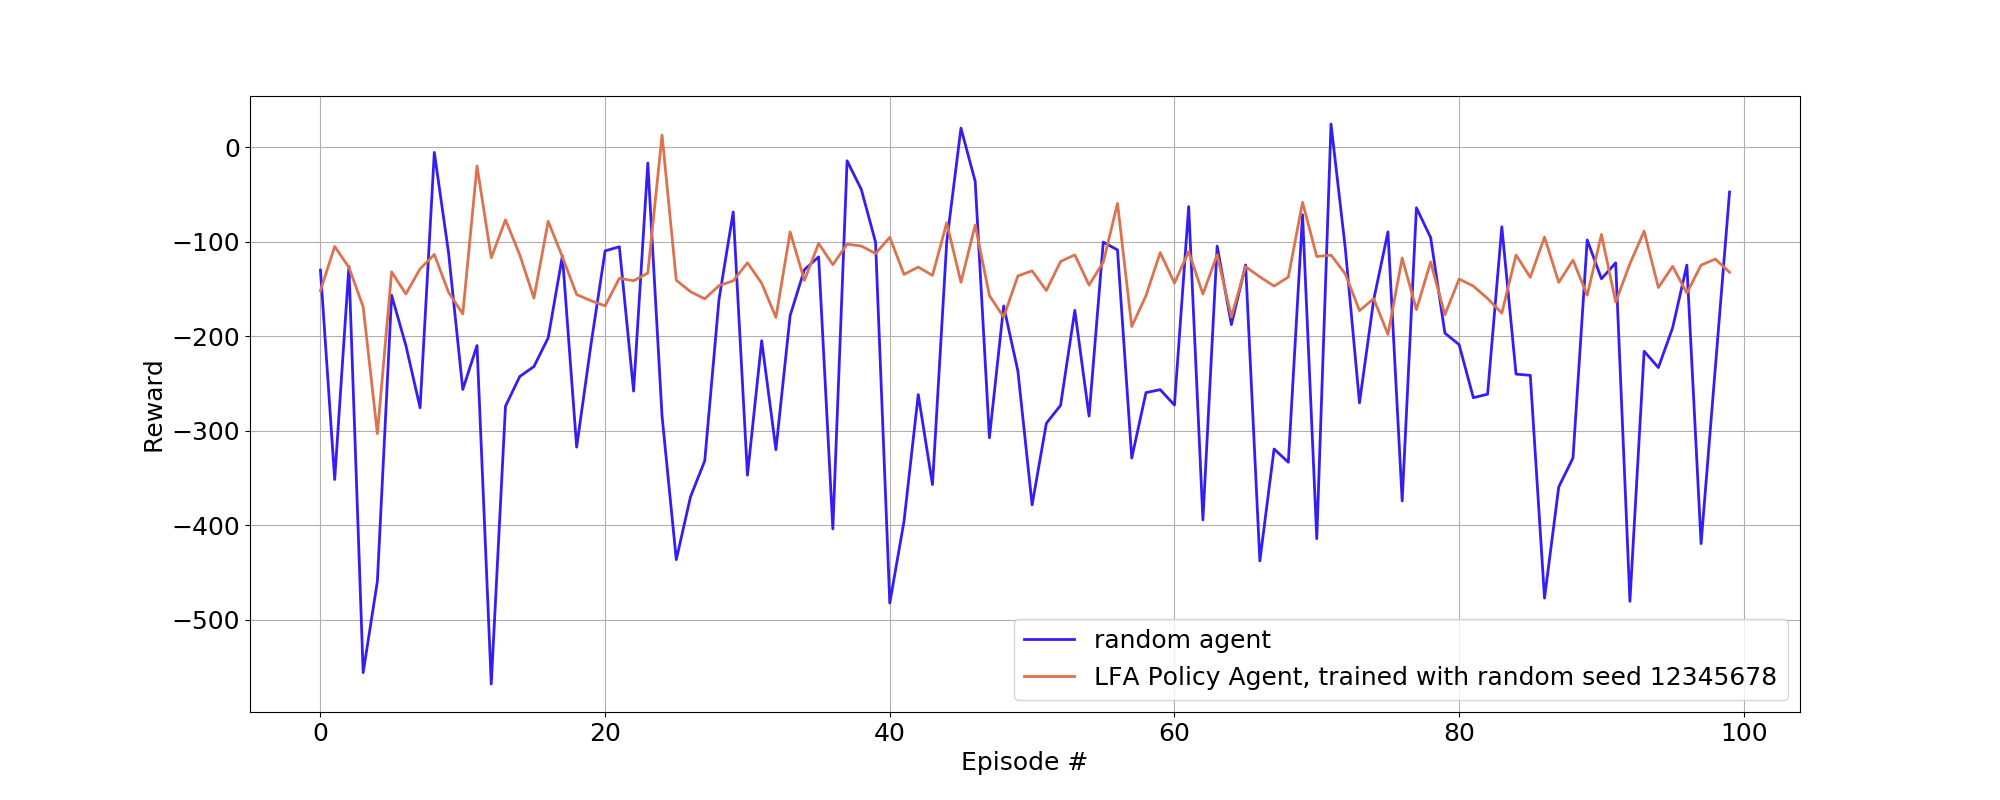
\includegraphics[width = 20cm]{12345678_eval.png}
		\caption{LFA Policy Agent, trained with random seed 12345678. Episode rewards after training.}
		\label{fig:4}
	\end{center}
	\end{figure}
	
\item Answer to question 4

Our neural network has an input layer with 8 units, two layers with 64 units, one layer with 16 units, and one output layer with 4 units. The four output units represent the two dimensional mean and the two dimensional standard deviation of the normal distribution over which we sample to choose the action. Training was done with a discount factor of 0.88 in order to stronger take returns into account that lay in the future. We experimentally determined the learning rate of the gradient descent step to 0.0001. 

\item Answer to question 5 (include 3 figures)

Figures \ref{fig:5} through \ref{fig:7} show the comparison between the three NN Policy Agents and the random agent.
\begin{figure}
	\begin{center}
		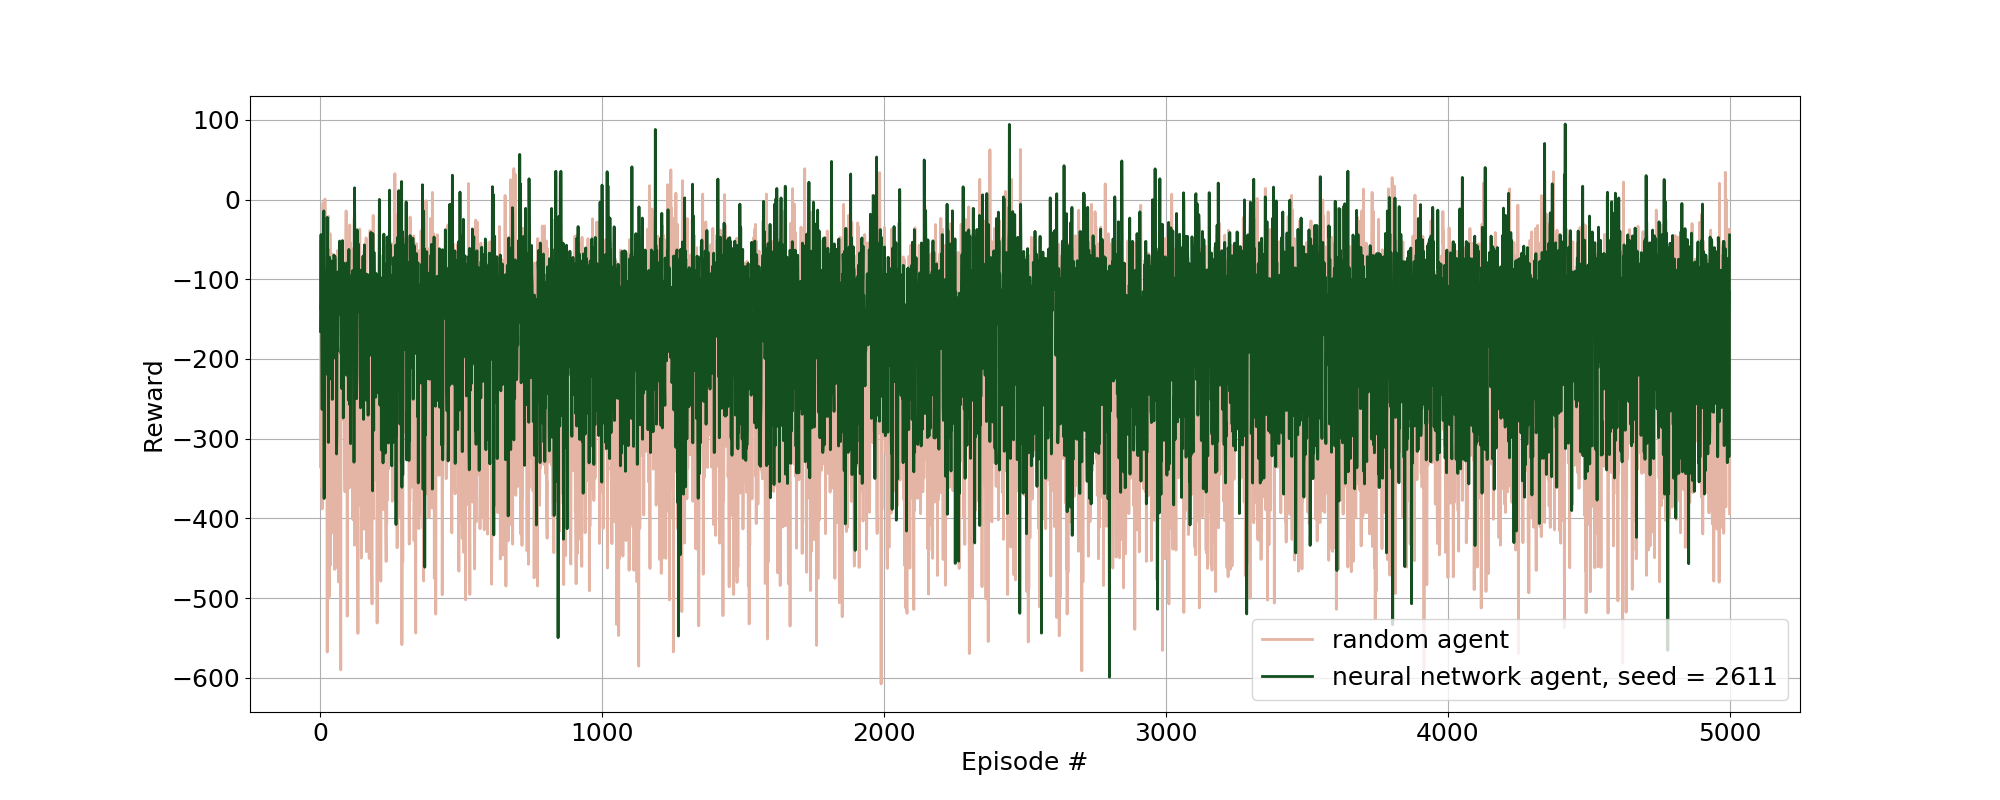
\includegraphics[width = 20cm]{nn_2611.png}
		\caption{LFA Policy Agent, trained with random seed 12345678. Episode rewards during training.}
		\label{fig:5}
	\end{center}
	\end{figure}

	\begin{figure}
	\begin{center}
		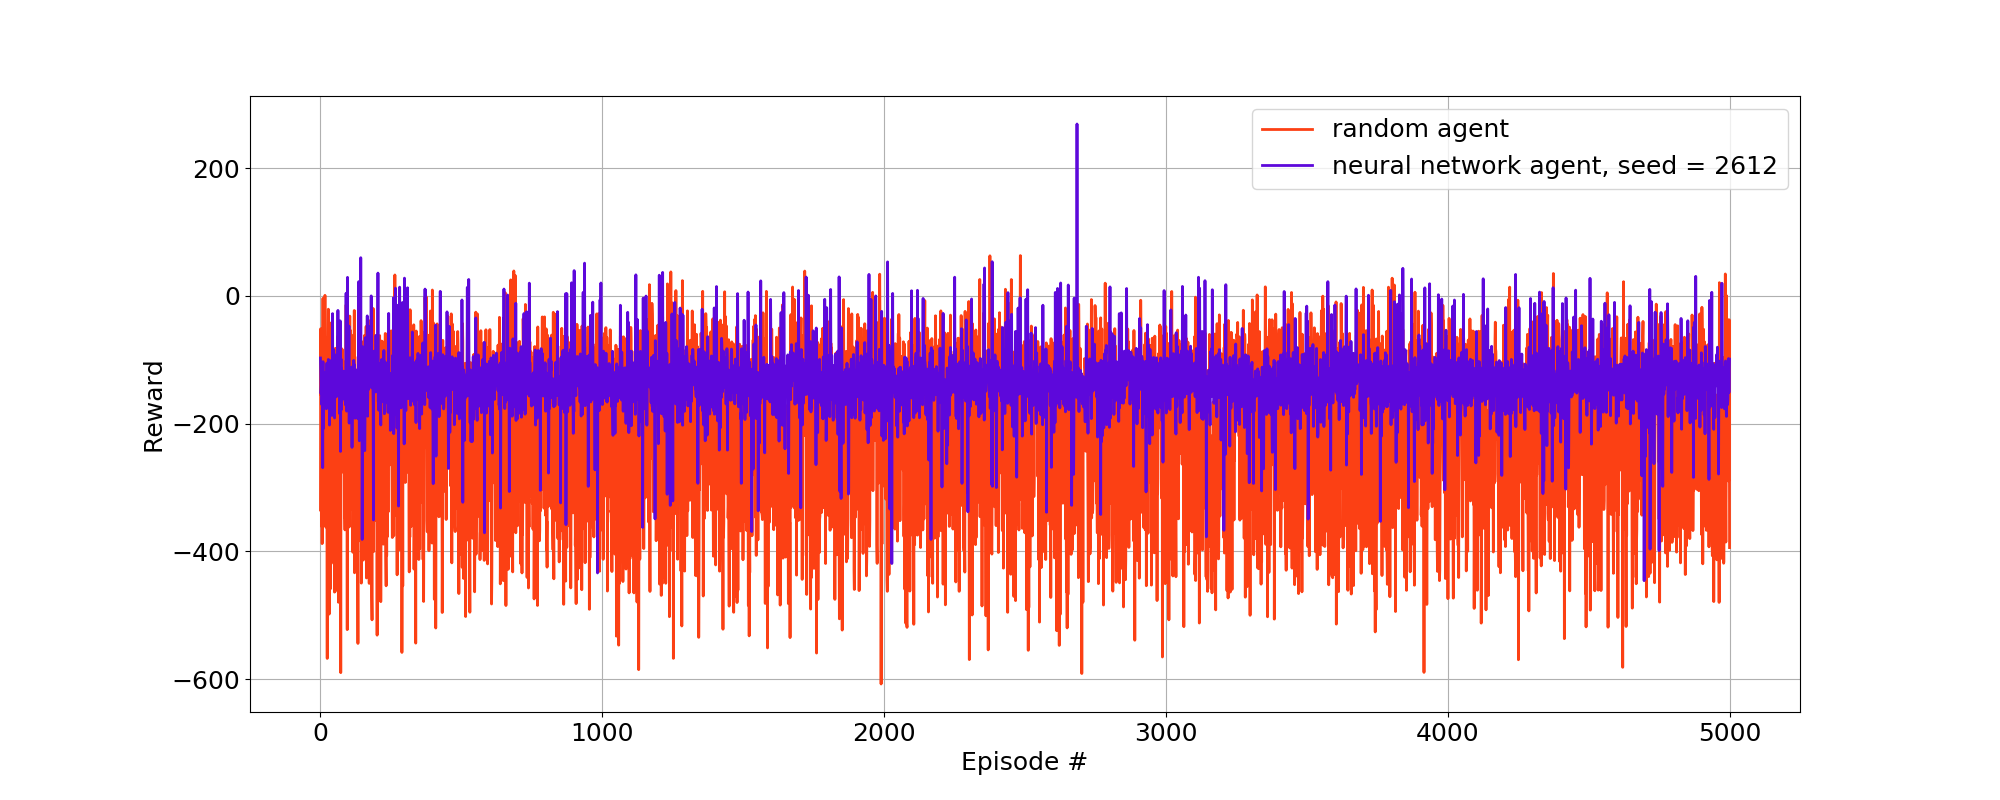
\includegraphics[width = 20cm]{nn_2612.png}
		\
		\caption{LFA Policy Agent, trained with random seed 2612. Episode rewards during training.}
		\label{fig:6}
	\end{center}
	\end{figure}
	\begin{figure}
	\begin{center}
		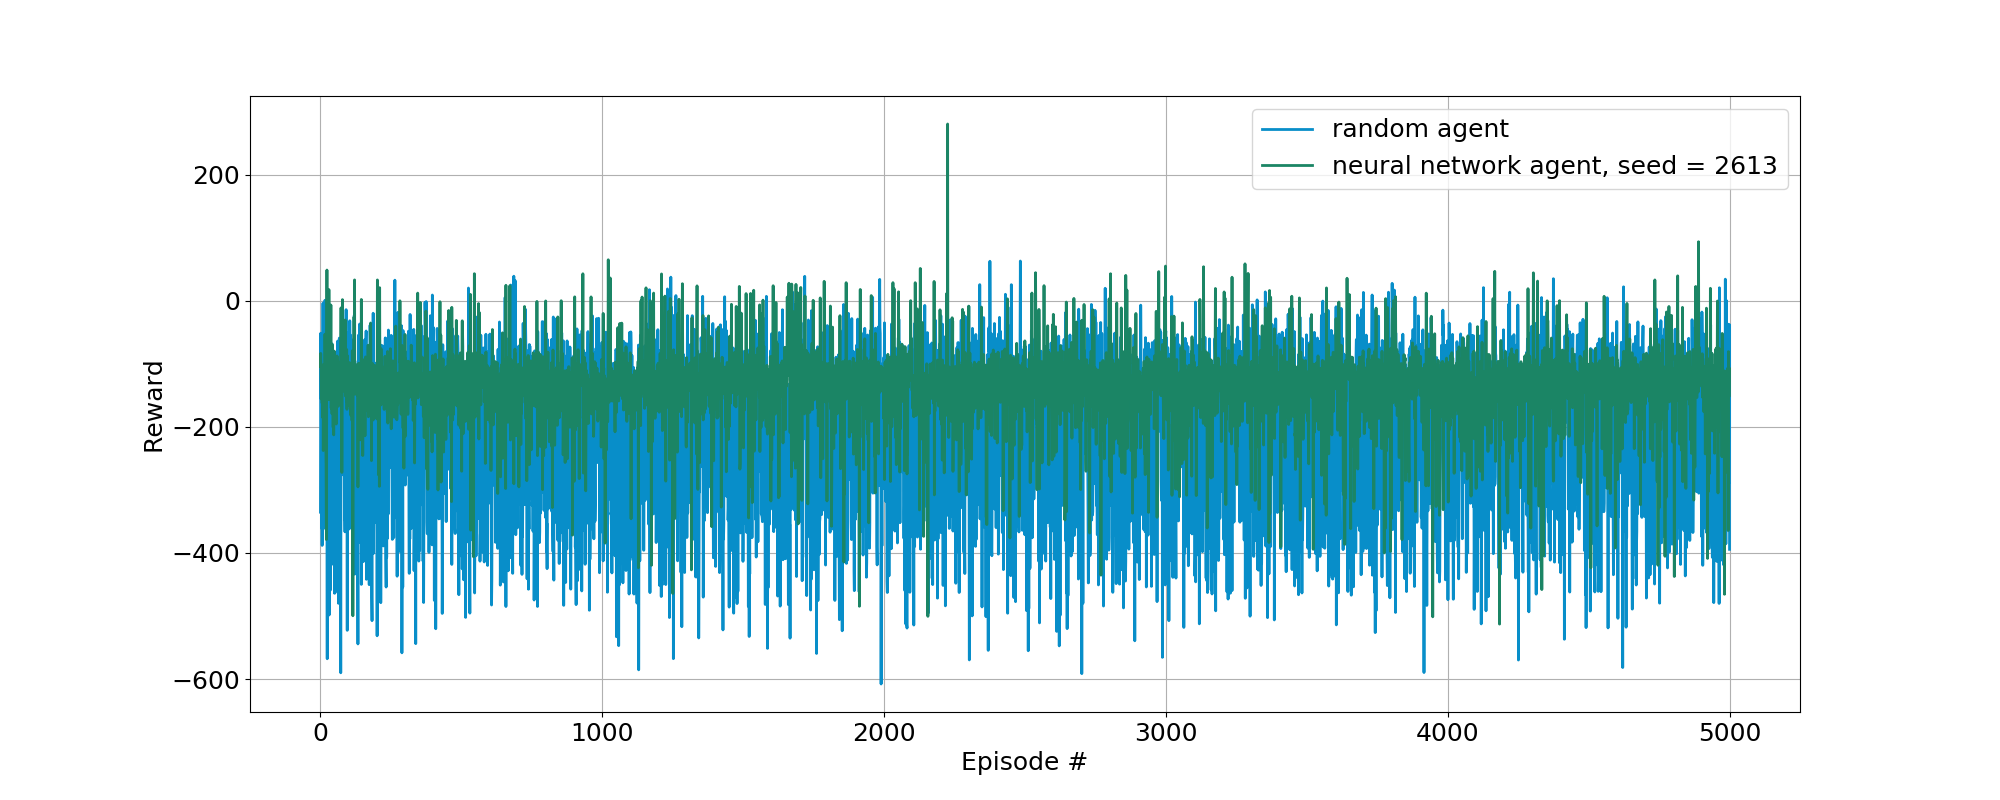
\includegraphics[width = 20cm]{nn_2613.png}
		\caption{LFA Policy Agent, trained with random seed 2613. Episode rewards during training.}
		\label{fig:7}
	\end{center}
	\end{figure}
	
\item Answer to question 6

The NN Policy Agent shows episodic rewards with a smaller variance than the episodic rewards of the random agent. However, maximal rewards do not exceed those of the random agent. We found that the hyperparameters strongly depend on each other and only very specific combinations yielded better than random results. Possibly a better architecture could achieve better results, however, deeper networks didn't improve in our tests.
\end{enumerate}

\end{document}
